\documentclass[12pt,twoside]{article}

\usepackage[scaled]{helvet}
\renewcommand\familydefault{\sfdefault} 
\usepackage[T1]{fontenc}
\usepackage[utf8]{inputenc}
\usepackage{sansmath}
%%%%%%%%%%%%%%%%%%%%%%%%%%%%%%%%%%%%%%%%%

\newcommand{\reporttitle}{Modelling the Effects of Projectile\\[0.5cm] Impact on Laminated Window Glass}
\newcommand{\reportauthor}{Michael Trapp}
\newcommand{\reportsupervisors}{John-Paul Latham, Jiansheng Xiang, Ado Farsi}
\newcommand{\reporttype}{\Huge Plan of Investigation}

%%%%%%%%%%%%%%%%%%%%%%%%%%%%%%%%%%%%%%%%%
% University Assignment Title Page 
% LaTeX Template
% Version 1.0 (27/12/12)
%
% This template has been downloaded from:
% http://www.LaTeXTemplates.com
%
% Original author:
% WikiBooks (http://en.wikibooks.org/wiki/LaTeX/Title_Creation)
%
% License:
% CC BY-NC-SA 3.0 (http://creativecommons.org/licenses/by-nc-sa/3.0/)
%-----------------------------------------------

\usepackage{textpos}
\usepackage[a4paper,hmargin=2.8cm,vmargin=2.0cm,includeheadfoot]{geometry}
\usepackage{ifxetex}
\usepackage{stackengine}
\usepackage{tabularx,longtable,multirow,subfigure,caption} %hang caption
\usepackage{fncylab} %formatting of labels
\usepackage{fancyhdr}
\usepackage{color}
\usepackage[ugly]{units}
\usepackage{url}
\usepackage{float}
\usepackage{csquotes}
\usepackage[english]{babel}
\usepackage{amsmath}
\usepackage{bm}
\usepackage{graphicx}
\usepackage[colorinlistoftodos]{todonotes}
\usepackage{epstopdf} % automatically replace .eps with .pdf in graphics
%\usepackage{backref}
\usepackage{array}
\usepackage{latexsym}
\usepackage{etoolbox}
\usepackage{enumerate} % for numbering with [a)] format 
\usepackage{enumitem}
\usepackage{tablefootnote}
\usepackage{booktabs}
\usepackage{tcolorbox}

% various theorems
\usepackage{ntheorem}
\theoremstyle{break}
\newtheorem{lemma}{Lemma}
\newtheorem{theorem}{Theorem}
\newtheorem{remark}{Remark}
\newtheorem{definition}{Definition}
\newtheorem{proof}{Proof}

% example-environment
\newenvironment{example}[1][]
{ 
\vspace{4mm}
\noindent\makebox[\linewidth]{\rule{\hsize}{1.5pt}}
\textbf{Example #1}\\
}
{ 
\noindent\newline\makebox[\linewidth]{\rule{\hsize}{1.0pt}}
}

\setlength{\parindent}{0em}  % indentation of paragraph
\setlength{\headheight}{14.5pt}
\pagestyle{fancy}
\fancyfoot[ER,OL]{\thepage}%Page no. in the left on, odd pages and on right on even pages
\fancyfoot[OC,EC]{\sffamily }
\renewcommand{\headrulewidth}{0.1pt}
\renewcommand{\footrulewidth}{0.1pt}
\captionsetup{margin=10pt,font=small,labelfont=bf}
\allowdisplaybreaks

%\usepackage{natbib}
\usepackage[sortcites,backend=biber,backref=true,hyperref=true,giveninits=true,maxbibnames=99,style=numeric,sorting=none,]{biblatex} 
\addbibresource{Bib.bib}
\usepackage{hyperref} % provide links in pdf
\hypersetup{
  pdftitle={},
  pdfsubject={}, 
  pdfauthor={\reportauthor},
  pdfkeywords={}, 
  pdfstartview=FitH,
  pdfpagemode={UseOutlines},
  bookmarksnumbered=true, 
  bookmarksopen=true, 
  colorlinks=true, 
  citecolor=blue,
  filecolor=blue, 
  linkcolor=blue, 
  urlcolor=blue,
  hypertexnames=true}

\begin{document}

\begin{titlepage}
%%%%%%%%%%%%%%%%%%%%%%%%%%%%%%%%%%%%%%%%%
%%%%%%%%%%%%%%%%%%%%%%%%%%%%%%%%%%%%%%%%%%%%%%%%%%%%%%%%
% Last modification: 2016-09-29 (Marc Deisenroth)
%%%%%%%%%%%%%%%%%%%%%%%%%%%%%%%%%%%%%%%%%%%%%%%%%%%%%%%%%%%%%%

\newcommand{\HRule}{\rule{\linewidth}{0.5mm}} % Defines a new command for the horizontal lines, change thickness here

%----------------------------------------------------------------------------------------
%	LOGO SECTION
%----------------------------------------------------------------------------------------


\includegraphics[width = 4cm]{imperial} 

\begin{center} % Center remainder of the page

%----------------------------------------------------------------------------------------
%	HEADING SECTIONS
%----------------------------------------------------------------------------------------
\vspace{1.5cm} 
\textsc{\LARGE \reporttype}\\[1.5cm] 
\textsc{\Large Imperial College London}\\[0.5cm] 
\textsc{\large Department of Earth Science and Engineering}\\[0.5cm] 
%----------------------------------------------------------------------------------------
%	TITLE SECTION
%----------------------------------------------------------------------------------------

\HRule \\[0.2cm]
{\huge \bfseries \reporttitle}\\ % Title of your document
\HRule \\[1.5cm]
\end{center}
%----------------------------------------------------------------------------------------
%	AUTHOR SECTION
%----------------------------------------------------------------------------------------

%\begin{minipage}{0.4\hsize}
\begin{flushleft} \large
\textit{Supervisors:}\\
\reportsupervisors\\[30pt]
\textit{Student:}\\
\reportauthor % Your name
\end{flushleft}
\vspace{2cm}
\makeatletter
Date: \@date 

\vfill % Fill the rest of the page with whitespace

\end{titlepage}

%%%%%%%%%%%%%%%%%%%%%%%%%%%% Main document
\section{Introduction}

Deliberate acts of terrorism, criminal activity and malicious behaviour pose significant threat to buildings and infrastructure. A recent state-of the arts review by \texttt{EU} decision makers revealed that current building guidelines tend to not take these threats into account. Appropriate regulations and guidelines require new experimental and numerical testing methods to accurately quantify the resilience of building elements against explosions events.

\bigbreak
The \texttt{AMCG} at \texttt{Imperial College London} recently developed a novel coupled dynamic gas/solid \texttt{FEMDEM} code, which is proposed to realistically simulate the shock wave impact on secondary laminated glass. In this paper, the code is provisionally applied to simulate \texttt{2D} and \texttt{3D} projectile impact on a single laminate. For verification, the results from each simulation are analysed and compared to experimental data from the literature.

\section{Physics Theory}

\subsection{Laminated Glass Model}

%Picture of Laminated Glass
%Measurements of the plies and inter-layer

Laminated glass is a sandwich structure consisting of two brittle glass plies and an adhered visco-elastic polymer inter-layer (or inter-face) in between. An optional back layer improves structural stability and additional energy absorption \cite{Bio10, Bra10}. The back layer traditionally consists of polycarbonate (\texttt{PC}) \cite{Bra10, Mon04}. Secondary laminated glass consists of two such laminates, separated by a layer of air.

\bigbreak
Advantageous properties of laminated glass include a relatively high penetration resistance \cite{Xu14}, low weight \cite{Wu14} and the adherence of fractured glass fragments to the structure to reduce the risk of injuries\cite{Xu14, Che17, Flo98, Ji98}. Breakage of the inner ply significantly reduces strength and facilitates a full collapse of the glass \cite{Flo98}.

\bigbreak
The exact prediction of crack initiation and propagation poses a significant challenge and requires ongoing research effort. Local stress intensification is provided by pre-existing micro-structural material flaws (so-called inhomogeneities or discontinuities) such as micro-cracks and voids \cite{Sch12}. Application of fracture stress $\sigma_{\rm{f}}$ causes these flaws to grow in size. \cite{Flo98, Pel16}.

\bigbreak
Many fracture models have been proposed. This paper uses the combined single and smeared crack model approach \cite{Mun99, Lat15}. According to the model, increasing stress leads to strain-hardening, followed by strain-softening. Strain-hardening can be modelled with continuum constitutive laws, as failure only occurs in the strain-softening part \cite{Mun13}. The constitutive law for the strain-hardening part is given by

\begin{equation}
    \tau=c+\sigma\,{\rm{tan}}\phi\,,
\end{equation}

with shear stress $\tau$, normal stress $\sigma$, cohesion $c$ and internal friction angle $\phi$. The stresses $\sigma$ and $\tau$ correspond to normal and shear displacements $\delta_{\rm{n}}$ and $\delta_{\rm{s}}$ and tensile and shear strengths $f_{\rm{t}}$ and $f_{\rm{s}}$. The material strengths are defined as the maximum strength in the stress-displacement diagram (fig. \ref{fig:FractureEnergy}), with maximum elastic displacement $\delta_{\rm{p}}$ and critical displacement $\delta_{\rm{s}}$.

\begin{figure}[!htbp]
    \centering
    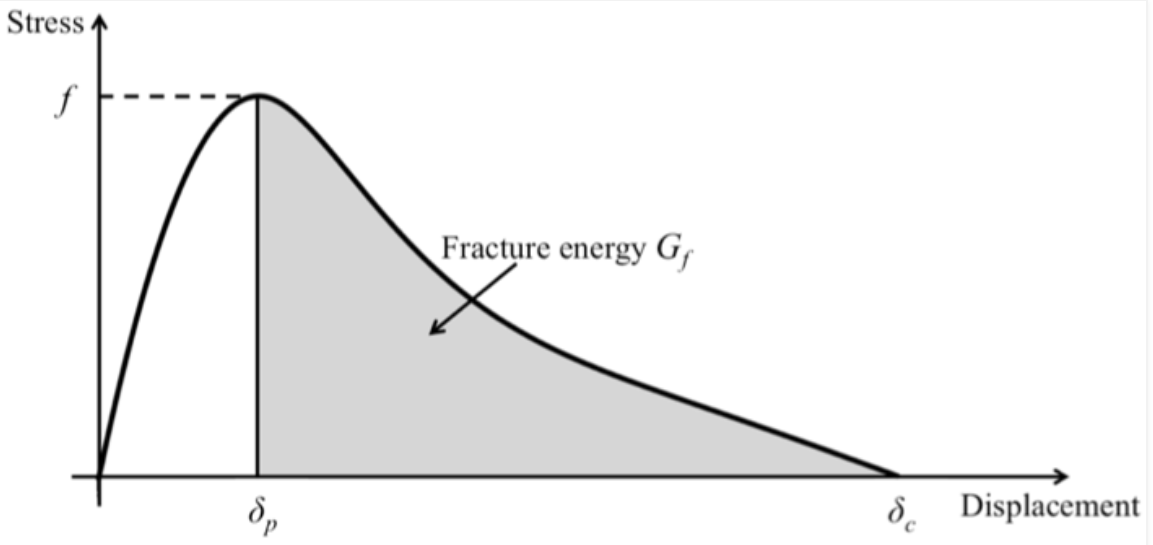
\includegraphics[width=\textwidth*2/3]{FractureEnergy}
    \caption{Stress-Displacement Curve. \cite{Lat15}}
    \label{fig:FractureEnergy}
\end{figure}

The fracturing in the strain-softening part is modelled using joint elements which are generated between two neighbouring shell elements. More comprehensive realisations of the model are carried out by Munjiza et al \cite{Mun04}, Lei et al \cite{Lei16} and Chen and Chang \cite{Che18}.

\subsection{Inter-layer Model}

The task of the inter-layer is the absorption of impact energy and the maintenance of adhesion to the plies \cite{Wu14}. Inter-layer materials include polymers such as traditional polyvinyl butyral (\texttt{PVB}), thermoplastic polyurethane (\texttt{TPU}), and most recently \texttt{SentryGlas}\textregistered Plus (\texttt{SGP}) \cite{Moh18, Wan18}. 

\bigbreak
Polymers are commonly modelled as hyper-elastic materials \cite{Gha15, Kim15}. Work done by stresses onto hyper-elastic materials only depends on the reference state $X$ and the current state $x$, but not on the load path (fig. \ref{fig:deformation}). Deformation from $X$ to $x$ is described by the deformation gradient \cite{Gu07}

\begin{equation}
    \label{eq:defgrad}
    F = \frac{{\rm{d}}\varphi}{{\rm{d}}X}
\end{equation}

with mapping function $\varphi$ from $X$ to $x$.

\begin{figure}[!htbp]
    \centering
    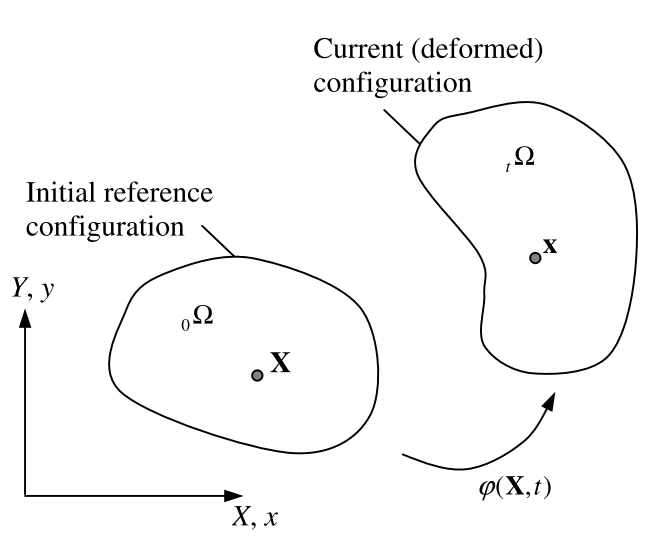
\includegraphics[width=\textwidth*2/3]{Deformation}
    \caption{Deformation from reference to current state. \cite{Gu07}}
    \label{fig:deformation}
\end{figure}

Hyper-elastics are mathematically described by a characteristic strain energy density function $W$. One of the simplest hyper-elastic models is the \texttt{Neo-Hookean} model \cite{Gha15}. Its characteristic strain energy potential function is given by

\begin{equation}
    \label{eq:NeoHooke}
    W=\frac{\mu_{\rm{0}}}{2}\left(I_{\rm{1}}-3\right)-\mu_{\rm{0}}\,{\rm{ln}}\,J+\frac{\lambda_{\rm{0}}}{2}{\rm{ln}}^2\,J\,,
\end{equation}

with Lam\'{e} constants $\lambda_{\rm{0}}$ and $\mu_{\rm{0}}$ from the linearised theory, $J=\lvert F\rvert$ and first invariant $I_{\rm 1}=C_{\rm{II}}$ with right Cauchy stress tensor \cite{Gha15}

\begin{equation}
    C_{\rm{ij}}=F_{\rm{Ii}}\,F_{\rm{Ij}}\,.
\end{equation}

Upper case indices refer to the reference configuration, while lower case indices refer to the current configuration.

\bigbreak
Another common, simple hyper-elastic model is the \texttt{Mooney - Rivlin} model \cite{Aba13, Kum16}. The characteristic strain energy function for the compressible 2-Parameter \texttt{Mooney - Rivlin} model \cite{Kum16} is given by

\begin{equation}
    \label{eq:MooneyRivlinSEF}
    W_{\rm{2}} = C_{\rm{10}}\left(\bar{I}_{\rm{1}}-1\right)+C_{\rm{01}}\left(\bar{I}_{\rm{2}}-1\right)+\frac{1}{d}\,(J-1)\,,
\end{equation}

where $C_{\rm{10}}$ and $C_{\rm{01}}$ are adjustable parameters, $d=2\,/\,K$ with bulk modulus $K$ and $\bar{I}_{\rm{1}}=J^{-\frac{1}{3}}\,I_{\rm{1}}$ and $\bar{I}_{\rm{2}}=J^{-\frac{1}{3}}\,I_{\rm{2}}$ are deviatoric invariants \cite{Aba13}.

\bigbreak
Other hyper-elastic models \cite{Aba13} include a more general polynomial model, \texttt{Arruda-Boyce}, \texttt{Ogden} and \texttt{Yeoh}. For the polynomial model, customized coefficients \cite{Sam19} already exist in the literature, specifically for laminated glass.

\bigbreak
Modelling the potential occurrence of fracture needs to be permitted for the inter-layer as well. This necessitates an extension of the smeared single and combined fracture model for the inter-layer.

\section{Numerics Theory}

\subsection{FEMDEM}
The combined discrete finite element method \texttt{FEMDEM} \cite{Wan18, Mun95, Mun99, Mun04, Mun12, Mun13, Guo16, Gao14, Xu14, Che18} is able to realistically model the deformation, interaction and fracturing of matrix bodies. The discrete elements consist of clusters of deformable finite elements. Cracks propagate along common finite element boundaries. Fracturing results in the formation of new discrete elements \cite{Mun13}. 

\bigbreak
Conventional \texttt{FEMDEM} methods are significantly inaccurate, as their applied complex shaped polygons require deformability restriction constraints (so-called locking) to maintain stability of the simulation \cite{Lat15}. 

\bigbreak
Munjiza et al \cite{Mun13} developed the novel \texttt{2D} \texttt{FEMDEM} code \texttt{Y}. The code is based on the so-called \texttt{F-bar} approach which uses 10-noded quadratic elements to reduce volumetric locking. Xiang et al \cite{Xia09} developed the novel \texttt{3D} \texttt{FEMDEM} code \texttt{Solidity}, \texttt{Y3D}, which features coupled multi-body interaction \cite{Lat15}.

\subsection{Governing Equations}
The governing equations for the finite element calculations in the \texttt{FEMDEM} method are the equations of motion. The equations are given by

\begin{equation}
    M\ddot{x}+\mu\dot{x}+f_{\rm{int}}=f_{\rm{ext}}=f_{\rm{l}}+f_{\rm{b}}+f_{\rm{c}}\,,
\end{equation}

with lumped nodal mass matrix $M$, nodal displacements $x$, viscosity $\mu$, internal nodal forces $f_{\rm{int}}$ and external nodal forces $f_{\rm{ext}}$. External forces contain consist of external loads $f_{\rm{l}}$, bonding forces $f_{\rm{b}}$ and contact forces $f_{\rm{c}}$. Internal forces $f_{\rm{int}}$ are generated by element deformation. FEMDEM systems solve these equations via explicit time integration using the forward \texttt{Euler} method \cite{Lei16}.

\subsection{Contact Algorithm}

The combination of discrete and finite elements is established via an interaction algorithm \cite{Lei16}. This algorithm consists of contact detection \cite{Che15} and contact interaction \cite{Mun13}. The contact forces between a contractor and target solid are given by

\begin{equation}
    f_c=\int_{\Gamma_{\rm{c}}}n\left(\varphi_{\rm{c}}-\varphi_{\rm{t}}\right)\,{\rm{d}}\Gamma_{\rm{c}}\,,
\end{equation}

with outward unit normal n to penetration boundary $\Gamma_{\rm{c}}$, and potential functions $\varphi_{\rm{c}}$ and $\varphi_{\rm{t}}$ for contractor and target. The contractor applies to the target a normal contact force

\begin{equation}
    f_n=-n\int_0^{L_{\rm{p}}} p\varphi(l){\rm{d}}l\,,
\end{equation}

with penetration length $L_{\rm{p}}$, potential function $\varphi$ along the target edge and penalty term $p$. It also applies a tangential friction force 

\begin{equation}
    f_{\rm{t}}=\mu_{\rm{mob}}\lVert f_{\rm{n}} \rVert\frac{v_{\rm{r}}}{\lVert v_{\rm{r}}\rVert}\,,
\end{equation}

with relative velocity $v_{\rm{r}}$ at the Gauss point and mobilised friction coefficient $\mu_{mob}$ which varies during the shearing process. A more detailed explanation is given by Lei et al \cite{Lei16}.

\subsection{Joint Constitutive Model}

 The joint constitutive model \cite{Lat15} introduces empirical micro-scale roughness effects to account for dilation and normal stiffness on stressed new and preexisting fracture surfaces.
 
 \bigbreak
 A more detailed explanation is given by Lei et al \cite{Lei16} and Chen and Chan \cite{Che18}.

\section{Numerical Model Approach}

\subsection{Setup}

A \texttt{2D} input \texttt{Y} file is generated using the pre-processor \texttt{GID} \cite{GID11}. The geometry could also be imported from common \texttt{CAD} software such as \texttt{AutoCAD}. The input file contains the model including the geometry, constraints, materials, as well as the simulation parameters. The high performance computing (\texttt{HPC}) system at \texttt{Imperial College London} is applied to generate time series images for the simulation. The series is analysed using the post-processing software \texttt{Hyperview} \cite{Hyp17}. For the \texttt{3D} simulation setup, which is is not considered for now, a similar approach will be applied.

\subsection{Parameters}

\begin{figure}[h!]
    \centering
    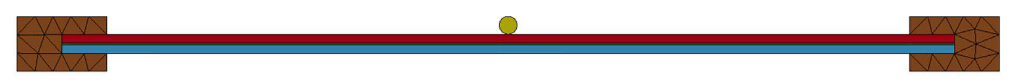
\includegraphics[width=\textwidth]{Geometry}
    \caption{\texttt{2D} geometry of the laminated glass structure and projectile \cite{Che18}}
    \label{fig:geometry}
\end{figure}

Fig. \ref{fig:geometry} illustrates the preliminary \texttt{2D} geometric setup. The figure shows the initial state of the spherical projectile (yellow) immediately before impact on the laminated glass (impactor glass plies in blue, inner glass ply in red, inter-layer in green). The glass is fixed via a support system (brown). The support structure is not modelled for now and is replaced with no-velocity boundary conditions acting on the sides of the glass plies. 

\bigbreak
In real-world applications, the dimensions of the inter-layer are smaller than the dimensions of the glass plies. Therefore, a translational degree of freedom in \texttt{y}-direction exists for the inter-layer. This effect will also need to be considered in this paper.

\bigbreak
Critical flaws, which cause complete structural failure, are usually found on the cut and machined glass edges \cite{Pel16}. Based on this consideration, the boundary structure layout requires special care. A project task remains to determine a realistic boundary structure to be applied.

\bigbreak
The majority of modelling parameters are adduced from the literature. A provisional list of material parameters is given in appendix \ref{ch:MaterialParameters}. A provisional list of input file simulation parameters is provided in appendix \ref{ch:SimulationParameters}.

\bigbreak
Modifications to this preliminary geometric setup will include changes to the shape of the projectile, as well as changes to the thickness of the layers. A potential consideration is to model the projectile as firearm ammunition instead of a circle (or sphere). A symmetry boundary condition may be applicable and only half of the laminate may need to be modeled.

\bigbreak
The dimensions of the glass plate is set to $2000\,{\rm{mm}}\times2000\,{\rm{mm}}$ in order to avoid anisotropic effects. The thickness of the glass plies is set to $2\,{\rm{mm}}$ and $0.76\,{\rm{mm}}$ for the inter-layer. For now, a \texttt{PVB} material is chosen for the inter-layer. Many models in the literature use similar dimensions, e.g. \cite{Mun04}.

\bigbreak
The preliminary mesh for all bodies consists of triangular elements. For the \texttt{3D} model, tetrahedral elements \cite{Che18} are to be considered. The preliminary element size is $1\,{\rm{mm}}$. Necessary modifications include reducing the number of elements for the projectile, as it is not of interest for the analysis and increasing the element size for far-field mesh elements for the plies and inter-layer. Potentially, differently shaped elements are more optimal for the results. The glass and inter-layers need to consist of several element layers to enable a more precise analysis. 

\bigbreak
The radius of the steel sphere (or circle) is set to $2.5\,{\rm{mm}}$. The volume of the spherical projectile is given by 

\begin{equation}
    V=\frac{4\pi}{3}r^3=\frac{4\pi}{3}\left(2.5\,{\rm{mm}}\right)^3\approx65.4\,{\rm{mm}}^3\,.
\end{equation}

The time step \cite{Far19} is set accordingly to

\begin{equation}
\Delta t=\sqrt{\frac{V\footnotemark\,\rho\footnotemark}{\rm{penalty\,\, number}}}=\sqrt{\frac{65.4\cdot7.8\cdot10^3}{4\cdot{10}^{11}}}\approx1\cdot{10}^{-6}{\rm{s}}
\end{equation}
\addtocounter{footnote}{-2}
\stepcounter{footnote}
\footnotetext{volume  $\left({\rm{in}}\,{\rm{mm}}^3\right)$ of the smallest element, without units}
\stepcounter{footnote}
\footnotetext{density $\left({\rm{in}}\,{\rm{kg}}/{\rm{m}}^3\right)$ of the material of the smallest element, without units}

To simulate real time $t=2\,{\rm{s}}$, the maximum number of time steps required \cite{Far19} is given by

\begin{equation}
    n_{\rm{t}}=\frac{t}{\Delta t}=\frac{2\,{\rm{s}}}{10^{-6}\,{\rm{s}}}=2\cdot10^6
\end{equation}

\subsection{Verification}

Numerical simulations need to be verified using data from physical experiments in order to draw conclusions on the degree of accuracy of the numerical model.

\bigbreak
Physical experiments involving the breakage of glass by projectiles or shock blasts require special safety arrangements. Air blast impact experiments are being conducted outdoors by service company \texttt{Jabisupra} \cite{Jab16} in cooperation with \texttt{Imperial College London}. The company is active in the field of envelope security and specialises in protecting infrastructure from certain threats. The data from \texttt{Jabisupra} is not expected to be ready and applicable for this project. Many other researchers have already conducted impact experiments in the past. A majority of the findings from these experiments are likely to be applicable to verify the model for this project.

\bigbreak
Dynamic impact on laminated glass comprises hard and soft body impact \cite{Moh17}. Hard body impact such as ballistic impact \cite{Bra10} causes minimal deformation to the projectile, while soft body impact such as bird impact \cite{Moh17} causes the projectile to undergo extensive deformation.

\bigbreak
Relevant parameters of the impact projectile include the normal velocity \cite{Gra98, Kar14, Dar13, Wu14}, the mass \cite{Kar14, Dar13}, the angle \cite{Gra98, Kar14, Dar13}, the shape \cite{Dar13} and the size \cite{Wu14}. Relevant parameters for the outer glass ply include its dimensions \cite{Wan18}, its mass, the support conditions \cite{Wan18} and the make-up \cite{Wan18}. For the inter-layer, the material \cite{Moh18, Wan18, Mon04}, thickness \cite{Ji98, Kar14, Wan18} and temperature \cite{Moh18, Zha19} are relevant.

\bigbreak
Low velocity ($\approx 20\,\mathrm{m}/\mathrm{s}$) hard impact experiments include the use of projectiles in form of road construction chippings \cite{Gra98}, ballistics \cite{Mon04}, drop-down weights \cite{Che15, Mil12, Wan18}, aluminum projectiles \cite{Mil12} and steel balls \cite{Beh99, Flo98, Wan18}. High velocity (around $180\, {\rm{m}}/{\rm{s}}$) soft impact experiments include the use of silicon rubber projectiles \cite{Moh17} and gas guns \cite{Moh18}.

\bigbreak
Wang et al \cite{Wan18} found that the panel size had an inferior effect on the breakage resistance \cite{Wan18}. Similarly, Monteleone et al \cite{Mon04} found that only a local area of the ply around the impact absorbed the impact energy for high velocities.

\bigbreak
Karunarathna \cite{Kar14} found that impact velocity and plate thickness contributed significantly towards the impact resistance, compared to impact mass and inter-layer thickness. Wang et al \cite{Wan18} found an increased inter-layer thickness to have a negative effect on energy absorption. Liu et al \cite{Liu16} established that the inter-layer thickness did not contribute towards energy absorption. Behr and Kremer \cite{Beh99} found an increased inter-layer thickness to better protect the inner ply. Kim et al \cite{Kim16} numerically optimised the \texttt{PVB} inter-layer constitution to prevent all damage to the inner glass ply.

\bigbreak
Liu et al \cite{Liu16} numerically investigated the optimisability of the inter-layer in terms of energy absorption by simulating the impact of a human head. Zhang et al \cite{Zha19} investigated the influence of temperature on the inter-layer and found that a hybrid \texttt{TPU}/\texttt{SGP}/\texttt{TPU} inter-layer performed best over the entire range of tested temperatures.

\section{Hypothesis}

The software Solidity is expected to realistically predict and quantify the solid-solid interaction, deformation and fracturing behavior of the laminated window glass upon impact with the projectile. Experimental data from previous research is adduced to further verify this hypothesis.

\section{Milestones}

{\color{red} due 28 June 2019}

\begin{enumerate}
    \item Compose Plan of Investigation (01-28 June)
    \item Review of Current Theory (01-21 June)
    \item Software Setup (21-28 June)
    \item Specification of Testing Procedures (21-28 June)
    \item First Prototype Programme (21-28 June)
\end{enumerate}

\vspace{0.3cm}
{\color{red} due 30 August 2019} 

\begin{enumerate}[resume]
    \item 2D Simulations (28 June - 12 July)
    \item 3D Simulations (12 July - 09 August)
    \item Validation/Verification of Results (09 August - 30 August)
    \item Outline of Report (28 June - 30 August)
    \item Final Draft of Report (01 June - 30 August)
\end{enumerate}

\vspace{0.3cm}
{\color{red} due early-mid September}

\begin{enumerate}[resume]
    \item oral presentation
\end{enumerate}

\newpage
%\bibliographystyle{unsrt}
%\setlength{\bibsep}{5.0pt}
\printbibliography
%\bibliography{Bib}
%
\appendix
\newpage
\section{Material Parameters}
\label{ch:MaterialParameters}

\begin{table}[!htbp]
  \begin{tabular}{llll}
    Property                                                & Glass             & PVB                   & Steel Projectile  \\\midrule            
    Density $\rho\,\left[{\rm{kg}} / {\rm{m}}^3\right]$     & 2500 \cite{Xu10}  & 1100 \cite{Xu10}      & 7800 \cite{Che18} \\
    Young's Modulus $E\,\left[{\rm{Pa}}\right]$             & 7e10 \cite{Xu10}  & 2.2e2 \cite{Ved17}    & 2e11 \cite{Che18} \\
    Poisson's Ratio $\nu$                                   & 0.22 \cite{Xu10}  & 0.49 \cite{Che15}     & 0.3 \cite{Che18}  \\
    Mass damping coefficient $\mu$                          & 0                 & 0                     & 0                 \\
    Elastic penalty term                                    & 7e10              & 2.2e2                 & 2e11              \\
    contact penalty                                         & 1.4e11            & 4.4e2                 & 4e11              \\
    Mode I energy rate $G_{\rm{I}}\,\left[{\rm{J}}/{\rm{m}}^2\right]$     & 10 \cite{Xu10}    &  2.8e3 \cite{Hoo17}    & 1.9e5 \cite{Sta00}\\
    Mode II energy rate $G_{\rm{II}}\,\left[{\rm{J}}/{\rm{m}}^2\right]$   & 50 \cite{Xu10}    &                       &     \\
    Mode III energy rate $G_{\rm{III}}\,\left[{\rm{J}}/{\rm{m}}^2\right]$ & 50 \cite{Xu10}    &                       &     \\
    Tensile Strength $\sigma \left[{\rm{Pa}}\right]$        & 6e7 \cite{Che15}  & 2e7 \cite{Zan12}      & 1e7 \cite{Wu14}   \\
    Internal friction coefficient                           & 0.1 \cite{Che15}  & 0.7 \cite{Kun15}      & 0.15 \cite{Sah07} \\
    Internal cohesion $\left[{\rm{Pa}}\right]$              & 7e10              & 2.2e2                 & 2e11              \\
    Pore fluid pressure $\left[{\rm{Pa}}\right]$            & 0                 & 0                     & 0                 \\
    Joint friction coefficient                              &                   &                       &                   \\
    Joint roughness coefficient $\texttt{JRC}_{\rm{0}}$ \tablefootnote{\label{note1}at laboratory conditions}   & & &       \\
    Joint compressive strength $\texttt{JCS}_{\rm{0}}$\textsuperscript{\ref{note1}}&                            & &         \\
    Joint sample size $\left[{\rm{m}}\right]$               &                   &                       &                   \\
    Interface friction                                      & 0.1 \cite{Che15}  & 0.62 \cite{Fah07}     & 0.44 \cite{Fah07} \\
    2D Problems                                             & plane stress & & \\\bottomrule
  \end{tabular}
  \caption{List of preliminary Y2 input material parameter values.}
  \label{tab:matpar}
\end{table}

\newpage
\section{Simulation Parameters}
\label{ch:SimulationParameters}

\begin{table}[!htbp]
  \begin{tabular}{ll}
    Parameter                               & Value                             \\\midrule  
    Maximum number of timesteps             & 2e6                               \\
    Current number of timesteps             & 0                                 \\
    Restart file saving frequency           & 1e2                               \\
    Gravity in \texttt{X} Direction (m/s2)  & 0                                 \\
    Gravity in \texttt{Y} Direction (m/s2)  & 0                                 \\
    Gravity in \texttt{Z} Direction (m/s2)  & -9.8                              \\
    Timestep (s)                            & 1e-6                              \\
    Output frequency                        & 10                                \\
    Current number of iterations            & 0                                 \\
    Gravity setting stage (s)               & 0                                 \\
    Load ramping stage (s)                  & 0                                 \\
    Maximum dimension (m)                   & 10                                \\
    Maximum force (N)                       & 1e6                               \\
    Maximum velocity (m/s)                  & 100                               \\
    Maximum stress (Pa)                     & 1e8                               \\
    Maximum displacement (m)                & 0.1                               \\
    Minimum joint aperture (m)              & 1e-7                              \\
    Maximum contacting couples              & 1e7                               \\
    Accuracy (bit)                          & 32                                \\
    Joint friction model                    & Coulomb                           \\
    Initial aperture correlation            & roughness                         \\\bottomrule
  \end{tabular}
  \caption{List of preliminary Y2D input simulation parameter values.}
  \label{tab:simpar}
\end{table}

%\newpage
%
%\begin{table}[h!]
%  \centering
%  \begin{tabular}{ll}
%    Parameter               & Description                       \\\midrule  
%    
%    \texttt{/YD/YDC/MCSTEP} & Maximum number of timesteps       \\
%    \texttt{/YD/YDC/NCSTEP} & Current number of timesteps       \\
%    \texttt{/YD/YDC/ISAVE}  & Restart file saving frequency     \\
%    \texttt{/YD/YDC/DCGRAX} & Gravity in \texttt{X} Direction   \\
%    \texttt{/YD/YDC/DCGRAY} & Gravity in \texttt{Y} Direction   \\
%    \texttt{/YD/YDC/DCGRAZ} & Gravity in \texttt{Z} Direction   \\
%    \texttt{/YD/YDC/DCSTEC} & Size of timestep                  \\
%    \texttt{/YD/YDC/DCTIME} & Current time                      \\
%    \texttt{/YD/YDC/DCURELX}& Not specified                     \\
%    \texttt{/YD/YDC/INITER} & Not specified                     \\
%    \texttt{/YD/YDC/ICOUTF} & Output frequency                  \\
%    \texttt{/YD/YDC/ICOUTI} & Current number of iterations      \\
%    \texttt{/YD/YDC/DCSIZC} &                                   \\
%    \texttt{/YD/YDC/DCSIZF} &                                   \\
%    \texttt{/YD/YDC/DCSIZS} &                                   \\
%    \texttt{/YD/YDC/DCSIZV} &                                   \\
%    \texttt{/YD/YDC/DCSIZD} &                                   \\
%    \texttt{/YD/YDC/DCSIZA} &                                   \\
%    \texttt{/YD/YDC/DCSTEC} &                                   \\
%    \texttt{/YD/YDC/DCTIME} &                                   \\
%    \texttt{/YD/YDC/DCRMPT} &                                   \\
%    \texttt{/YD/YDC/DCGRST} &                                   \\
%    \texttt{/YD/YDC/ICSAVF} &                                   \\
%    \texttt{/YD/YDC/ICOUTP} &                                   \\
%    \texttt{/YD/YDC/ICFMTY} &                                   \\
%    \texttt{/YD/YDC/ICIATY} &                                   \\\bottomrule
%  \end{tabular}
%  \caption{List of preliminary Y2D input simulation parameter values}
%  \label{tab:inpar}
%\end{table}

\end{document}